%\documentclass[10pt]{beamer} % aspect ratio 4:3, 128 mm by 96 mm
\documentclass[10pt,aspectratio=169]{beamer} % aspect ratio 16:9

%\graphicspath{{../../figures/}}
\graphicspath{{figs/}{../../figures/}{../../../reports/figures/png/}}
%\includeonlyframes{frame1,frame2,frame3,frame4,frame5,frame6,frame7,frame8,frame9}
%\includeonlyframes{frame10,frame11,frame12,frame13}
%\includeonlyframes{frame14,frame15,frame16,frame17,frame18,frame19,frame20,frame21}
%\includeonlyframes{frame22,frame23,frame24,frame25,frame26}
%\includeonlyframes{frame27,frame28}
%%%%%%%%%%%%%%%%%%%%%%%%%%%%%%%%%%%%%%%%%%%%%%%%%%
% Packages
%%%%%%%%%%%%%%%%%%%%%%%%%%%%%%%%%%%%%%%%%%%%%%%%%%
\usepackage{appendixnumberbeamer}
\usepackage{booktabs}
\usepackage{pgfplots}
\usepackage{xspace}
\usepackage{amsmath}
\usepackage{multirow}
\usepackage{totcount}
\usepackage{tikz}
\usepackage[T1]{fontenc}
\usepackage{ragged2e}

\usepackage{wrapfig}
%\usepackage{comment}
%\usetikzlibrary{external} % speedup compilation
%\tikzexternalize % activate!
%\usetikzlibrary{shapes,arrows}  

%\usepackage{bibentry}
%\nobibliography*
\usepackage{caption}%
\captionsetup[figure]{labelformat=empty}%
%%%%%%%%%%%%%%%%%%%%%%%%%%%%%%%%%%%%%%%%%%%%%%%%%%
% Metropolis theme custom modification file
\input{metropolis_mods.tex}
%%%%%%%%%%%%%%%%%%%%%%%%%%%%%%%%%%%%%%%%%%%%%%%%%%
% Custom commands
%%%%%%%%%%%%%%%%%%%%%%%%%%%%%%%%%%%%%%%%%%%%%%%%%%
% matrix command 
\newcommand{\matr}[1]{\mathbf{#1}} % bold upright (Elsevier, Springer)
%\newcommand{\matr}[1]{#1}          % pure math version
%\newcommand{\matr}[1]{\bm{#1}}     % ISO complying version
% vector command 
\newcommand{\vect}[1]{\mathbf{#1}} % bold upright (Elsevier, Springer)
% bold symbol
\newcommand{\bs}[1]{\boldsymbol{#1}}
% derivative upright command
\DeclareRobustCommand*{\drv}{\mathop{}\!\mathrm{d}}
\newcommand{\ud}{\mathrm{d}}
% 
\newcommand{\themename}{\textbf{\textsc{metropolis}}\xspace}
%%%%%%%%%%%%%%%%%%%%%%%%%%%%%%%%%%%%%%%%%%%%%%%%%%
%  Title page options
%%%%%%%%%%%%%%%%%%%%%%%%%%%%%%%%%%%%%%%%%%%%%%%%%%
 \date{}
%%%%%%%%%%%%%%%%%%%%%%%%%%%%%%%%%%%%%%%%%%%%%%%%%%
% option 1
%%%%%%%%%%%%%%%%%%%%%%%%%%%%%%%%%%%%%%%%%%%%%%%%%%
\title{Odpowiedzi do pytań i uwag zawartych w recenzji z~dnia 11~czerwca~2023 dra hab. inż. Łukasza Jankowskiego, prof. IPPT PAN}
\author{\textbf{Piotr Fiborek}}
% logo align to Institute 

\institute{Institute of Fluid Flow Machinery\\Polish Academy of Sciences \\ \vspace{-1.5cm}\flushright{\includegraphics[width=4cm]{logo_eng_40mm.eps}}}
%%%%%%%%%%%%%%%%%%%%%%%%%%%%%%%%%%%%%%%%%%%%%%%%%%
\begin{document}
	%%%%%%%%%%%%%%%%%%%%%%%%%%%%%%%%%%%%%%%%%%%%%%%%%%
	\maketitle
\begin{frame}[label=frame1]{Komentarz 1}\justifying
	\textit{Przedstawione wyniki są wartościowe i bardzo interesujące badawczo. Recenzentowi jednak
	nieco brakuje choćby krótkiej dyskusji potencjalnego scenariusza zastosowania praktycznego.
	Wartości zaproponowanych wskaźników uszkodzenia wydają się być bardzo zależne od
	konkretnej konfiguracji geometrycznej. Czy dla każdego zastosowania konieczna by była
	ponowna kalibracja modelu numerycznego? Jeśli tak, to czy kalibracja przeprowadzona dla
	elementu w stanie nieuszko\-dzonym byłaby wystarczająca?}
\end{frame}
\begin{frame}[label=frame2]{Komentarz 1}\justifying
	\textcolor{blue}{W przypadku zastosowania praktycznego zapropnowanycej metody, konieczna jest kalibracja dla każdorazowej konfiguracji geometrycznej czy materiałowej. Kalibracja jedynie w stanie nieuszko\-dzonym byłaby niewystarczająca, ponieważ wartości parametrów materiałowych stosowanych komponentów (CFRP, czujniki PZT) silnie zależą od warunków brzegowych panujących w trakcie pomiaru. W pracy przedstawiono zależność MADIF od temperatury otoczenia, ale wpływ na~funkcje może mieć również wilgotność powietrza, naprężenia konstrukcji oraz starzenie materiałów.\\
	W związku z powyższym, zarys praktycznego zastosowania metody przedstawia się następująco:
	\begin{itemize}
		\item \textcolor{blue}{Identyfikacja stałych materiałowych struktury}
		\item \textcolor{blue}{Opracowanie modelu}
		\item \textcolor{blue}{Wyznaczenie MADIF}
		\item \textcolor{blue}{Pomiar monitorowanej konstrukcji}
		\item \textcolor{blue}{Przetwarzanie sygnału wraz z kompensacją z uwagi na panujące warunki otoczenia}
		\item \textcolor{blue}{Odczytanie wielkości uszkodzenia z MADIF}
	\end{itemize}}
\end{frame}

\begin{frame}[label=frame3]{Komentarz 2}\justifying
	\textit{W rozdziale 4.5 opisany jest model tłumienia. Jest to model tłumienia środowiskowego: macierz tłumienia jest proporcjonalna do macierzy mas. Doktorant wystarczająco uzasadnia taki wybór aspektami numerycznymi i powołaniem się na literaturę. Recenzentowi brakuje jednak konkretnej wartości współczynnika proporcjonalności: ile on wynosił i w jaki sposób był wyznaczony?}
\end{frame}
\begin{frame}[label=frame4]{Komentarz 2}\justifying
\textcolor{blue}{Wartość współczynnika proporcjonalności macierzy tłumienia została ustalona poprzez dostrojenie odpowiedzi modelu referencyjnego do pomiarów eksperymentalnych. Wartości tłumienia zostały dostosowane indywidualnie tylko dla płyty CFRP w zależności od każdej z częstotliwości wymuszenia. Wartości współczynnika były różne dla przemieszczeń w kierunku osi X i Y, które w~głównej mierze odpowiadają za tłumienie modu S0, oraz dla kierunku osi Z, który jest związany z tłumieniem modu A0. Dla symulacji próbek z uszkodzeniami oraz analizy wpływu temperatury otoczenia przyjęto wartości referencyjne, które przedstawione są w Tabeli \ref{tab:damp}.
\begin{table}[!hbt]
	\tabcolsep=0.1cm
	\centering
	\caption{\label{tab:damp} Wpspółczynniki tłumienia dla płyty CFRP}
	\begin{tabular}{cccc}
		\textbf{Frequency} & \multicolumn{3}{c}{\(\alpha_M\times 10^3\)} \\
		\([\mathrm{kHz}]\) & x & y & z\\\midrule
		50 & 1 & 1 & 5\\
		100 & 10 & 10 & 24\\
		150 & 50 & 50 & 500
	\end{tabular}
\end{table}
}
\end{frame}	

\begin{frame}[label=frame5]{Komentarz 3}\justifying
\textit{Rozdział 4.10 i Rysunek 4.6 ilustruje m.in. przyspieszenie obliczeń w stosunku do algorytmu benchmarkowego. Czy wartości referencyjne zostały otrzymane na tym samym komputerze, co~zaproponowana metoda, czy też czas obliczeń został wzięty z literatury?}\\
\textcolor{blue}{Tak, obliczenia przeprowadzono na tym samym komputerze.}
\end{frame}

\begin{frame}[label=frame6]{Komentarz 4}\justifying
\textit{Rozdział 5.6 opisuje testy zbieżności opracowanego modelu numerycznego.
(\textbf{a}). Nie jest do końca jasne, w jaki sposób wyliczany jest wskaźnik zaproponowany zależnością (5.2). Czy symbole \(e^{max}\) i \(e^p\) oznaczają maksymalne wartości obwiedni? Jeśli jednak są to wartości chwilowe, to we wzorze prawdopodobnie brakuje znaku sumy lub całki.}\\
\textcolor{blue}{(\textbf{a}) \(e^{max}\) jest to obwiednia sygnału wyznaczononego dla modelu o elementach zdefiniowanych za~pomocą wielomianu o~największym stopniu \((p=11)\). W celu uniknięcia niejasności interpretacyjnych, wskaźnik powinien być zdefiniowany zgodnie z poniższym.}
\begin{columns}
	\column{0.5\textwidth}
	\begin{alertblock}{Wskaźnik użyty w pracy}
	\begin{eqnarray}
		\delta^{\mathrm{conv}} = \frac{\sum{\left(e_n^{\mathrm{max}}-e_n^{p}\right)^2}}{\sum{\left(e_n^{max}\right)^2}} \times 100\%\nonumber,
	\end{eqnarray}
	\end{alertblock}
\column{0.5\textwidth}
	\begin{alertblock}{\textcolor{green}{Wskaźnik poprawiony}}
		\begin{eqnarray}
			\delta^{\mathrm{conv}} = \frac{\sum_{n=1}^{N}{\left(e_n^{\mathrm{p=11}}-e_n^{p=p_i}\right)^2}}{\sum_{n=1}^N{\left(e_n^{p=11}\right)^2}} \times 100\%\nonumber,
		\end{eqnarray}
	\end{alertblock}

\end{columns}
\textcolor{blue}{gdzie: $e_n^{p=p_i}$ jest to wartość obwiedni sygnału w chwili $n$ obliczony  dla elementów o stopniu \(p_i = [4,\,5,\,7,\,9]\).}
\end{frame}

\begin{frame}[label=frame7]{Komentarz 4}\justifying
\textit{(\textbf{b}) W Tabeli 5.3 brakuje wiersza odpowiadającego częstotliwości 150 kHz. Dobrze by było to~wyjaśnić w tekście – w tym miejscu rozprawy nie jest to jasne dla Czytelnika.}\\
\textcolor{blue}{(\textbf{b}) Jest to moje niedopatrzenie wynikające z faktu, iż mod A0 dla częstotliwości 150 kHz nie~był wykorzystywany w analizie wyznaczenia MADIF. Jednakże Czytelnik na obecnym etapie nie~jest jeszcze o tym poinformowany, więc Tabela 5.3. powinna zawierać wartości również dla~tej częstotliwości.}
\begin{table}[H]
	\small
	\tabcolsep=0.5cm
	\centering
	\begin{tabular}{cccccc}
		\toprule
		\textbf{Propagation angle} & \(0^{\circ}\) & \(30^{\circ}\) & \(45^{\circ}\) & \(60^{\circ}\) & \(90^{\circ}\)\\
		\textbf{Frequency} [kHz] & \multicolumn{5}{c}{\textbf{Wavelength} [mm]}\\
		\midrule
		50 & 16.5 & 15.2 & 15.0 & 15.2 & 16.6\\
		100 & 10.3 & 9.6 & 9.5 & 9.6 & 10.3\\
		\textcolor{red}{150} & \textcolor{red}{7.5} & \textcolor{red}{7.1} & \textcolor{red}{7.0} & \textcolor{red}{7.1} & \textcolor{red}{7.5}\\
		\bottomrule
		\multicolumn{6}{r}{{\scriptsize{source: Dispersion Calculator v1.9}}}
	\end{tabular}
\end{table}
\end{frame}

\begin{frame}[label=frame8]{Komentarz 4}\justifying
	\begin{wrapfigure}{r}{0.5\textwidth}
		\centering
		\includegraphics[width=0.4\textwidth]{figs/dx_100kHz_1600us}
		\label{fig:conv_x}
	\end{wrapfigure}
\textit{(\textbf{c}) Testy zbieżności przestrzennej przeprowadzono z wykorzystaniem przebiegów czasowych w zakresie do 250 us (Rysunek 5.6a). Jednak w dalszej części rozprawy symulacje są przeprowadzane dla znacznie dłuższych odcinków czasowych (do 1600 us). Czy krzywe otrzymane dla p=7,9,11 pokrywałyby się również dla dłuższych odcinków czasowych?}

\textcolor{blue}{(\textbf{c}) Zgadza się, że dla dokładności analizy należałoby zbadać zbieżność dla sygnałów o takiej samej długości, jakie zostały wykorzystane w dalszej części dysertacji. Jednakże krzywe zbieżności prezentują podobne wzorce, jak w przypadku krótszych sygnałów. Na rysunku obok przedstawiono sygnał referencyjny oraz o elementach wielomianu stopnia \(p=7\).}
\end{frame}
\begin{frame}
	\begin{figure}
		\centering
		\includegraphics[width=\textwidth]{figs/dx_conv_1600us}
	\end{figure}
\end{frame}
\begin{frame}[label=frame9]{Komentarz 4}\justifying
\begin{wrapfigure}{r}{0.5\textwidth}
	\centering
	\includegraphics[width=0.5\textwidth]{figs/dt_50kHz_400us}
\end{wrapfigure}

\textit{(\textbf{d}) Rozdział 5.6.2: Jaki krok czasowy został ostatecznie wykorzystany podczas obliczeń? Czytelnikowi nieco też brakuje porównania (na dłuższych odcinkach czasowych) przebiegów obliczonych dla paru długości kroku czasowego (poniżej wartości krytycznej), podobnie jak to miało miejsce na Rys. 5.6a dla różnych wartości p.}\\
\textcolor{blue}{(\textbf{d}) Ostatecznie wybrano \(\Delta t=9.155\) ns, taki sam dla trzech wybranych częstotliwości. Na~rysunku obok zaobserwować można, że~wraz ze spadkiem wartości kroku czasowego sygnał jest niezmienny.}
\end{frame}

\begin{frame}[label=frame10]{Komentarz 5}\justifying
\textit{Rozdział 6.3: walidacja eksperymentalna przeprowadzona z wykorzystaniem lasera
skanującego i~pełnego pola prędkości (Rys. 6.7-12) jest interesująca i przekonująca, lecz ma charakter głównie wizualny i jakościowy. Czy możliwe byłoby wprowadzenie pewnych miar ilościowych? Jakie mogłyby to być miary?}
\textcolor{blue}{Sekcja mogłaby być uzupełniona o miary ilościowe wykorzystane w~walidacji za pomocą PZT, czyli pomiar prędkości i amplitudę pierwszej paczki. Obie wielkości można określić w funkcji kąta propagacji fali. Możnaby wyznaczyć współczynniki tłumienia poszczególnych modów oraz krzywe dyspersji analizowanego panelu, analizując pełne pole dla wzbudzenia sygnałem szerokopasmowym.
Dodatkowo dla pełnego pola propagacji możnaby obliczyć wskaźniki wykorzystane w opracowaniu MADIF:
\begin{eqnarray}
	\mathrm{RMSD} & = & 1 - \sqrt{\frac{\sum_{i=1}^{L}\left(e_{num}-e_{exp}\right)^2}	{\sum_{i=1}^{L}e_{exp}^2}},\nonumber\\
	\mathrm{CC} & = & \frac{L\sum_{i=1}^{L}e_{num}e_{exp}-\sum_{i=1}^{L}e_{num}\sum_{i=1}^{L}e_{exp}}{\sqrt{L\sum_{i=1}^{L}e_{num}^2-\left[\sum_{i=1}^{L}e_{num}\right]^2}\sqrt{L\sum_{i=1}^{L}e_{exp}^2-\left[\sum_{i=1}^{L}e_{exp}\right]^2}}.\nonumber
\end{eqnarray}
}
\end{frame}

\begin{frame}[label=frame11]{Komentarz 6}\justifying
\textit{Rozdział 6.4: walidacja z wykorzystaniem czasowych przebiegów odpowiedzi czujników 	opiera się głównie na maksymalnej amplitudzie i czasie jej przybycia (ToF). Wydaje się jednak, że te dwa wskaźniki relatywnie łatwo jest dostroić numerycznie (przynajmniej w pewnym zakresie) poprzez zmiany współczynnika tłumienia oraz procentowej zawartości włókien w modelowanym materiale warstwy zewnętrznej. Czy nie byłoby wskazane wprowadzenie dodatkowych wskaźników jakości obejmujących dłuższe odcinki czasowe symulowanej i zmierzonej odpowiedzi, a nie wyłącznie piki obwiedni? Byłoby to zgodne z dwoma ostatecznie wybranymi wskaźnikami uszkodzenia, które są wyliczane na podstawie całego okna czasowego, a nie jedynie głównego piku.}\\
\textcolor{blue}{Walidacji modelu dokonano poprzez porównanie prędkości i amplitudy modów bezpośrednio przesłanych z transmitera do czujnika, które mają decydujący wpływ na dokładność dopasowania sygnału z symulacji i sygnału z eksperymentu. Zgadzam się, że wprowadzenie dodatkowych wskaźników jakości, które obejmują dłuższe odcinki czasowe symulowanej i zmierzonej odpowiedzi, byłoby wartościowym uzupełnieniem analizy. Skupienie się na całym oknie czasowym, może dostarczyć bardziej reprezentatywnych informacji, które uwzględniają, błędy obliczeń numerycznych, tłumienie oraz dyspersje propagującej fali na dłuższym odcinku oraz ewentualne konwersje modów na krawędzi struktury.}
\end{frame}

\begin{frame}
\textcolor{blue}{W tabeli poniżej znajdują się wartości wskaźników RMSD i CC dla odpowiadających częstotliwości. W przypadku doskonałego dopasowania sygnału numerycznego, wskaźniki przyjmują wartość jeden, zatem najlepsze wyniki uzyskano dla wskaźnika CC, szczególnie w~przypadku częstotliwości 150 kHz.}
	\begin{table}[H]
		\small
		\tabcolsep=0.5cm
		\centering
		\begin{tabular}{ccc}
			\toprule
			\textbf{Frequency} [kHz] & RMSD & CC\\
			\midrule
			50 & 0.43 & 0.60\\
			100 & 0.54 & 0.82\\
			150 & 0.63 & 0.94\\
			\bottomrule
		\end{tabular}
	\end{table}

\end{frame}
\begin{frame}[label=frame12]{Komentarz 7}\justifying
\textit{Rozdział 7.1: ostatecznie wyznaczone wskaźniki są obliczane na podstawie sygnału o pełnej długości. Jaka to jest długość i jak została ona wyznaczona? Wydaje się, że tej informaticji nie~ma~w~tekście podanej wprost.}\\
\textcolor{blue}{Zdecydowanie zabrakło informacji o długości sygnału, pozostawiając Czytelnikowi w domyśle odczytanie jej z wykresu Figure 7.1. Na podstawie prędkości modu A0 dla 50 kHz, przyjęto czas w jakim pik modu A0 pokona drogę od transmitera do krawędzi panelu a następnie po~odbiciu trafi do czujnika. Dla odległości 500 mm i prędkości modu 926 m/s długość sygnału po~zaokrągleniu wynosi 600 us. Dla pozostałych częstotliwości przyjęto tę samą długość sygnału co w przypadku wymuszenia o częstotliwości 50 kHz.}
\end{frame}

\begin{frame}[label=frame13]{Komentarz 8}\justifying
\textit{Rozdział 7.1, proponowane wskaźniki uszkodzenia (zależności 7.2 – 7.7):
(\textbf{a}) Proponowane wskaźniki mają nieco zróżnicowany charakter. Na przykład w wypadku	\(e^H = e^D\) (brak uszkodzenia) P2P jest równe zero, lecz pozostałe wskaźniki są równe 1. W miarę różnicowania się \(e^D\) od \(e^H\), wartości niektórych wskaźników mogą rosnąć, innych maleć, a jeszcze innych rosnąć lub maleć. Być może dobrze by było zwrócić na to uwagę w tekście. (\textbf{b}) Wartości pierwszych trzech wskaźników (P2P, SAPS i SAPR) są ze sobą związane w sposób deterministyczny.\\}

\textcolor{blue}{(a, b) Faktycznie, jest to istotny aspekt do uwzględnienia, gdyż może wpłynąć na zrozumienie ostatecznych wyników. Należałoby dokładniej omówić poszczególne wskaźniki, np. wstawiajac (na str. 73 po drugiej linijce od góry) następujący fragment: \textit{The reference value of the P2P is set to zero, while the other indicators begin at one. However, due to the complex phenomena occurring in wave propagation within the panel, such as wave reflections from the edge of defects or wave leakage, it is challenging to determine the monotonicity of the indices in advance.}}
\end{frame}
\begin{frame}[label=frame14]{Komentarz 8}\justifying 
(\textbf{c}) W kontekście dwóch powyższych uwag wydaje się, że zdanie porównujące wielkości wskaźników otrzymanych dla S0 i A0 (str.74, 4–5 linia tekstu od góry) nie jest do końca uzasadnione.
\textcolor{blue}{(\textbf{c}) Prównując wskaźniki należałoby doprecyzować, a wskazane zdanie (\textcolor{black}{The S0-based DIs values are also less than the A0-based signals,	except the RMSD at 50 kHz.}) zastąpić przez: \textit{Except for full-length 50 kHz RMSD, the indices for the damage range analysed are undetermined. For S0 windowed signals, some are very insensitive to changes in the size of the damage, especially P2P 50 kHz, P2P, SAPS, ENG, CC 100 kHz and CC 150 kHz.
In the case of the A0-windowed signals, negligible changes are shown for both CC and SAPR at 100 kHz, whereas minimal changes are seen for SAPR at 100 kHz for full-length signals.}}
\end{frame}	

\begin{frame}[label=frame15]{Komentarz 9}\justifying
\textit{Str. 81 i Rys. 7.12: podane rozbieżności rozmiarów uszkodzenia są bardzo niewielkie, lecz dotyczą odległości pomiędzy aproksymowanymi krzywymi. Odległości rzeczywistych punktów
pomiarowych są znacznie większe. Błąd wyznaczenia rozmiaru uszkodzenia w praktyce zależy nie tylko od błędu systematycznego krzywej, lecz również od rozrzutu pomiarów wokół krzywej. Czy nie należałoby zwrócić na to uwagę w tekście?}\\
\textcolor{blue}{Zgodzam się, że należałoby uwypuklić różnice w odległościach pomiędzy aproksymowanymi krzywymi a~rzeczywistymi punktami pomiarowymi, ponieważ wartości te mają bezpośredni wpływ na~dokładność wyznaczania rozmiaru uszkodzenia.
W przypadku RMSD błąd wynosi odpowiednio \(\Delta w=[22.8,\,3.6,\,2.4,\,8.4,\,-6.0,\,\emptyset]\), przy czym nie można wyznaczyć największego uszkodzenia, ponieważ wartość pomiaru jest poza skalą MADIF. W przypadku CC błąd wynosi odpowiednio \(\Delta w=[10.8,\,-6.0,\,-12.0,\,-13.2,\,-24.0,\,\emptyset]\), ostatni pomiar w tym przypadku również leży poza skalą MADIF.}
\end{frame}
\begin{frame}
		\begin{figure}
			\centering
			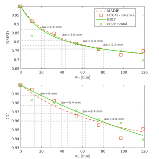
\includegraphics[width=0.5\textwidth]{figs/MADIF_20}
		\end{figure}
\end{frame}
\begin{frame}[label=frame16]{Komentarz 10}\justifying
\textit{Rys. 8.3b: wydaje się, że przypadek (5) różni się od przypadku (6) jedynie symetrią (odbicie względem poziomej osi symetrii). Otrzymane z symulacji obwiednie jednak istotnie się różnią.	Dlaczego?}\\
\textcolor{blue}{Oś symetrii występuje jedynie w układzie lokalnym komórki rdzenia. W układzie globalnym panelu symetria nie występuje ponieważ czujniki PZT zlokalizowane są poza osią symetrii płyty. W 120 us sygnału oprócz modu A0 dochodzą również dwa mody S0 (odbicia od lewej i prawej krawędzi panelu), które różnią się od siebie z uwagi na brak symetrii globalnej. Aby uniknąć niejasności, w opisie symulacji powinien pojawić się komentarz o położeniu przetworników w~układzie globalnym panelu. Różnice występują w oknie czasowym A0, w którym rejestrowane są odbicia modu S0 od bocznych krawędzi panelu. W pierwszym oknie czasowym takie róznice nie~wy\-stępują, ponieważ jest~to~bezpośredni sygnał modu S0 rejestrowany przez czujnik.}
\end{frame}

\begin{frame}
	\begin{figure}
		\centering
		\includegraphics[width=\textwidth]{figs/pzt_placement}
	\end{figure}
\end{frame}
\begin{frame}[label=frame17]{Komentarz 11}\justifying

\textit{Wydaje się, że wiele wykresów w rozprawie powinno przedstawiać ten sam bazowy przebieg obwiedni. Dotyczy to na przykład Rys. 6.16b, Rys. 8.3(0) i Rys. 8.4(100\%). Jednak przebiegi się różnią. Dlaczego? To samo pytanie dotyczy też przebiegów samych pików przedstawionych np. na Rys. 8.4(100\%) i Rys. 8.5(100\%).}\\
\textcolor{blue}{Przebieg obwiedni z Rys. 6.16b różni się od pozostałych, ponieważ w tym przypadku współrzędne przetworników wynoszą \((x_1;y_1) = (-100;0) \) i \(x_2,y_2 = (+100;0)\) , natomiast w studium parametrycznym czujniki dopasowane są do komórek rdzenia i w przypadku (0) współrzedne wynoszą \((x_1;y_1) = (-104.304; -2.0)\) i \((x_2;y_2) = (+100.750; -2.0)\). W Rys. 8.4 niestety wystapił błąd w wykresie, gdzie jest błędna kolejność linii.}

\end{frame}

\begin{frame}
	\begin{columns}
		\column{0.5\textwidth}
		\begin{figure}
			\centering
			\caption{Wykres użyty w dysertacji}
			\includegraphics[width=\textwidth]{figs/pzt_d}
		\end{figure}
		\column{0.5\textwidth}
		\begin{figure}
			\centering
			\caption{Wykres poprawny}
			\includegraphics[width=\textwidth]{figs/pzt_d_new}
		\end{figure}
	\end{columns}
\end{frame}


\begin{frame}[label=frame18]{Komentarz 12}\justifying
\textit{Analiza wrażliwości przedstawiona w Rozdziałach 8.2.1–8.2.3 dotyczy przebiegów obwiedni. Czy można na podstawie wyników tej analizy wyciągnąć jakieś wnioski dotyczące wrażliwości MADIF?}\\
\textcolor{blue}{Analizowane parametry można podzielić na dwie kategorie: te które są niezmienne w czasie analizowanego okresu oraz te, które mogą ulec zmianie pod wpływem panujących warunków otoczenia, lub z powodu starzenia się komponentów konstrukcji. Do pierwszej grupy należą, wielkości geometryczne rdzenia, zawartość włókien węglowych, lokalizacja czujników, do drugiej natomiast zaliczane są parametry materiałowe komponentów. Parametry pierwszej grupy są~jednakowe zarówno dla stanu referencyjnego, jak i dla stanów w czasie monitorowania konstrukcji, zatem nie będą miały one wpływu na ewentualną zmianę przebiegu MADIF w czasie. Natomiast wrażliwość MADIF na zmianę pozostałych parametrów można zaobserwować w analizie zmiennej temperatury otoczenia.}
\end{frame}
\begin{frame}[label=frame18]{Uwagi techniczne i redakcyjne}\justifying
	\begin{itemize}
		\item Str. 22: we wzorze 4.5 siła jest oznaczona symbolem \(f_{ext}\) (mała litera), a w akapicie poniżej wzoru symbolem \(F_{ext}\) (wielka litera). Ta rozbieżność to prawdopodobnie literówka. \textcolor{blue}{Zgadza się, prawidłowy symbol to \(f_{ext}\).}
		\item Str. 32: czy „transfered matrix” nie powinno być zastąpione „transformed matrix”? \textcolor{blue}{Zgadza się, powinno być „transformed matrix”.}
		\item W Rozdziale 4.8: stabilność algorytmu całkowania numerycznego to nie jest niezależność od kroku czasowego (w tekście: „stable, i.e., independent of the time step”). To określenie należałoby zmodyfikować. \textcolor{blue}{Zdanie} \textit{"The time discretisation \(\beta = 0.25\) and \(\gamma = 0.5\) , is second-order accurate and the algorithm is a stable, i.e., independent of the time step."} \textcolor{blue}{powinno być zastąpione przez: "The time discretisation \(\beta = 0.25\) and \(\gamma = 0.5\), is second-order accurate and the algorithm is unconditionally stable, i.e., the solution behaves consistently regardless of the time step value."}
		\item  \small{Na str. 45 wysokość uszkodzenia podana jest jako 170 mm, natomiast na str. 57 jako 175 mm. Któraś z tych wartości powinna być skorygowana. \textcolor{blue}{Poprawna wartość uszkodzenia to 170 mm}}
		\item \small{Na str.45 pojawia się etykieta systemu LaTeX: „(fig:disbond)”. \textcolor{blue}{Zabrakło znacznika (\(\backslash\)ref\{fig:disbond\}) w pliku źródłowym .tex}}
	\end{itemize}
	
\end{frame}	
\end{document}